\begin{Problem}
	Sei
	\begin{align*}
&		f:\R\times \R\backslash \{0\} \to \R, (x,y)\to \frac{x^2}{y^2},\\
&		A:=\left\{ (x,y)\in \R^2|0\le y\le x, 0\le x \le 2, xy\ge 1 \right\} .
	\end{align*}
	Bestimmen Sie $\int_A f\dd{\lambda_2}$.
\end{Problem}
\begin{proof}
	Zuerst zeigen wir: $f$ ist messbar. Wir betrachten dazu $\{f< \alpha\} ,\alpha\in \R,\alpha >0$ (Wenn $\alpha\le 0$ ist die Menge die Leermenge, weil $f\ge 0$ stets). Es gilt dann
	\begin{align*}
		x^2<& \alpha y^2\\
		|x|<&\sqrt{\alpha}|y|
	\end{align*}
	Dann ist $\{f<\alpha\} $ eine Borelmenge, also $f$ ist messbar.

	Ähnlich wie in Übungen 8.2 ist $A$ eine Borelmenge. Die dritte Voraussetzung kann umgeformt werden:
	\begin{align*}
		y\ge& 1 / x\\
		x \ge& y \ge 1 / x
	\end{align*}
	was nur möglich ist, wenn $2\ge x\ge 1$ und in diesem Fall ist der Schnitt $\{y|(x,y)\in A\} $ nichtleer. Also wir berechnen das Integral über die Teilmenge nach der Präsenzübung
	\begin{align*}
		\int_A f\dd{\lambda_2}=&\int_{[1,2]}\int_{A_x} f\dd{\lambda_1}\\
		=&\int_1^2 \int_{1 / x}^x \frac{x^2}{y^2}\dd{\lambda_1(y)}\dd{\lambda_1(x)}\\
		=&\int_1^2 -x^2 y^{-1}|_{1 / x}^x\dd{\lambda_1(x)}\\
		=&\int_1^2 x^2\left( x-\frac{1}{x} \right) \dd{\lambda_1(x)}\\
		=& \left.\frac{x^4}{4}-\frac{x^2}{2}\right|_1^2\\
			=&\frac{9}{4}.\qedhere
	\end{align*}
\end{proof}
\begin{Problem}
	Sei
	\[
	A:=\left\{ (x,y,z)\in \R^3|x^2+y^2\le 1,\frac{1}{2}(x+y)^2+z^2\le 1 \right\} 
	.\] 
	Bestimmen Sie $\lambda_3(A)$.

	{\footnotesize \emph{Hinweis: Rotation}}
\end{Problem}
\begin{proof}
	$A$ ist eine Borelmenge und daher messbar. Wir schreiben $A_z$. Es gilt
	\begin{align*}
		1\ge& \frac{1}{2}(x+y)^2+z^2\\
		2(1-z^2)\ge& (x+y)^2\\
		|x+y|\le& \sqrt{2} \sqrt{1-z^2} 
	\end{align*}
	\begin{center}
		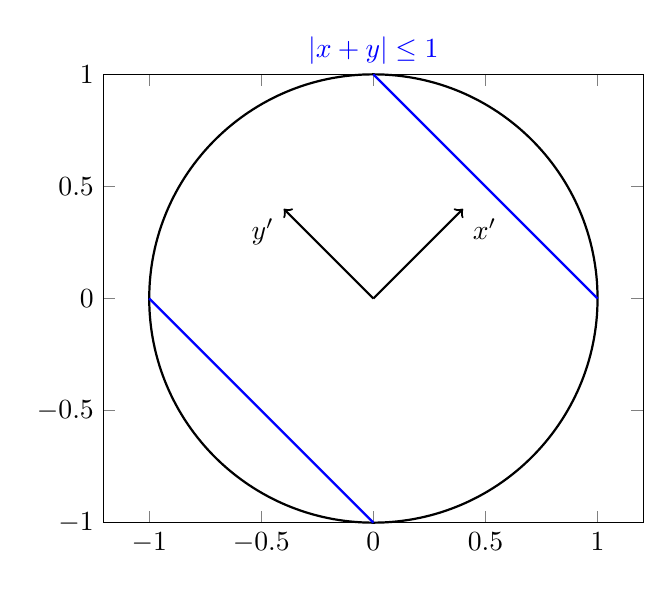
\begin{tikzpicture}
			\begin{axis}[xmin=-1,xmax=1,ymin=-1,ymax=1,axis equal,clip=false]
			\draw[thick] (axis cs: 0,0) circle (1);
			\addplot[domain=0:1,blue,thick] {1-x};
			\addplot[domain=-1:0,blue,thick] {-1-x};
			\draw (axis cs:0,1) node[anchor=south,blue] {$|x+y|\le 1$};
			\draw[thick,->] (axis cs:0,0) -- (axis cs:0.4,0.4);
			\draw[thick,->] (axis cs:0,0) -- (axis cs:-0.4,0.4);
			\draw (axis cs: 0.4,0.4) node[anchor=north west] {$x'$};
			\draw (axis cs:-0.4,0.4) node[anchor=north east] {$y'$};
			\end{axis}
		\end{tikzpicture}
	\end{center}
	Wir rotierenden dann das Koordinatensystem wie im Diagramm.
	\begin{center}
		\begin{tikzpicture}
			\begin{axis}[xmin=-1.15,xmax=1.15,ymin=-1.15,ymax=1.15,xlabel=$x'$,ylabel=$y'$, axis equal,clip=false,axis lines = center, y label style={anchor=south}, x label style ={anchor=west},scale=1.5,xtick={-1,-0.5,0,0.5,1},ytick={-1,-0.5,0,0.5,1}]
				\draw[thick] (axis cs:0,0) circle (1);
				\draw[thick,blue] (axis cs:{1/sqrt(2)},{-1/sqrt(2)}) -- (axis cs:{1/sqrt(2)}, {1/sqrt(2)});
				\draw[thick,blue] (axis cs:{-1/sqrt(2)},{-1/sqrt(2)}) -- (axis cs:{-1/sqrt(2)}, {1/sqrt(2)});
			\fill (axis cs:0,0) circle (1pt);
				\draw[thick] (axis cs:0,0) -- (axis cs:{1/sqrt(2)},{1/sqrt(2)});
				\draw (axis cs:{1/sqrt(2)},{1/(2*sqrt(2))}) node[anchor=east] {$|z|$};
				\fill[pattern=north east lines,pattern color=blue] (axis cs:{1/sqrt(2)},{1/sqrt(2)}) arc(45:0:1) -- (axis cs:{1/sqrt(2)},0) -- cycle;
				\fill[pattern=north east lines,pattern color=orange] (axis cs:{1/sqrt(2)},{-1/sqrt(2)}) arc(-45:0:1) -- (axis cs:{1/sqrt(2)},0) -- cycle;
				\fill[pattern=north east lines, pattern color=orange] (axis cs:{-1/sqrt(2)},{1/sqrt(2)}) arc(135:225:1) -- cycle;
				\draw (axis cs:{1/(2*sqrt(2))},0) node[anchor=south] {$\sqrt{1-z^2} $};
			\end{axis}
		\end{tikzpicture}
	\end{center}
	Das Maß der blauen Region ist
	\[
		\frac{1}{2}\sin^{-1}|z|-\frac{1}{2}|z|\sqrt{1-z^2} 
	,\]
	also das Maß von $A_z$ ist
	\begin{align*}
		\lambda_2(A_z)=&\pi(1)^2-4\cdot\frac{1}{2}\left( \sin^{-1}|z|-|z|\sqrt{1-z^2}  \right)\\
		=&\pi-2\left( \sin^{-1}|z|-|z|\sqrt{1-z^2}  \right) 
	\end{align*}
	Dann ist
	\begin{align*}
		\lambda_3(A)=&\int_{-1}^1 \pi-2(\sin^{-1}|z|-|z|\sqrt{1-z^2} \dd{z}\\
		=&2\int_0^1 \pi-2(\sin^{-1}|z|-|z|\sqrt{1-z^2} \dd{z}\\
		=&2\int_0^1\pi-2(\sin^{-1}z-z\sqrt{1-z^2}) \dd{z}\\
		=&2\left[ \int_0^1 \pi\dd{z}-2\int_0^1\sin^{-1}z\dd{z}+2\int_0^1 z\sqrt{1-z^2} \dd{z} \right]\\
		=&2\left[ \pi-2\int_0^1 \sin^{-1}z\dd{z}+2\int_0^1 z\sqrt{1-z^2} \dd{z} \right]. 
	\end{align*}
	Nebenrechnung:
	\begin{align*}
		\int_0^1 \sin^{-1}z\dd{z}=&z\sin^{-1}z|_0^1-\int_0^1 \frac{z}{\sqrt{1-z^2} }\dd{z}\\
		=&\frac{\pi}{2}-\int_0^1 \frac{z}{\sqrt{1-z^2} }\dd{z}\\
		u=&1-z^2,\qquad \dd{u}=-2z\dd{z}\\
		\int_0^1\sin^{-1}z\dd{z}=&\frac{\pi}{2}+\frac{1}{2}\int_1^0 \frac{1}{\sqrt{u} }\dd{u}\\
		=&\frac{\pi}{2}+\sqrt{u}|_1^0\\
		=&\frac{\pi}{2}-1\\
		\int_0^1 z\sqrt{1-z^2} \dd{z}=&-\frac{1}{2}\int_1^0 \sqrt{u} \dd{u}\\
		=&\frac{1}{2}\int_0^1 \sqrt{u} \dd{u}\\
		=&\frac{1}{3}u^{3 / 2}|_0^1\\
		=&\frac{1}{3}
	\end{align*}
	Eingesetzt:
	\begin{align*}
		\lambda_3(A)=&2\left[ \pi-2\left( \frac{\pi}{2}-1 \right) +\frac{2}{3} \right] \\
		=&2\pi-4\left( \frac{\pi}{2}-1 \right) +\frac{4}{3}\\
		=&2\pi-2\pi+4+\frac{4}{3}\\
		=&\frac{16}{3}.\qedhere
	\end{align*}
\end{proof}
\begin{Problem}
	Sei $S\in \R^{n\times n}$ ein invertierbare Matrix und $a\in \R^n$. Definere damit die Abbildung $\varphi:\R^n\to \R^n, x\to a+Sx$. Sei außerdem $A\in \mathcal{L}(n)$ und $f:\R^n\to \R$ $\mathcal{L}(n)-B^1$ messbar, sodass $\chi_{\varphi(A)}f$ $\lambda_n$ integrierbar ist. Zeigen Sie, dass dann $\chi_A(f\circ \varphi)$ $\lambda_n$-integrierbar ist mit
	\[
		\int_{\varphi(A)}f\dd{\lambda_n}=|\text{det}(S)|\int_A (f\circ\varphi) \dd{\lambda_n}
	.\] 
	{\footnotesize \emph{Hinweis: Lemma 2.92}}
\end{Problem}
\begin{proof}
	Nach Satz 1.83 und Bewegungsinvarianz ist $\varphi(A)$ messbar mit Maß $\lambda_n(\varphi(A))=|\text{det}(S)|\lambda_n(A)$. $\chi_{\varphi(A)}$ ist dann messbar. Weil $\varphi$ affin ist, ist $\varphi$ stetig und daher messbar. Dann ist $f\circ\varphi$ messbar, und als Produkt von messbare Funktionen ist $\chi_A(f\circ \varphi)$ $\lambda_n$-messbar.

	Wir verwenden Lemma 2.93 und betrachten $f^+$. Es gilt
	\begin{align*}
		\int_{\varphi(A)}f^+\dd{\mu}=&\int f^+\chi_{\varphi(A)}\dd{\mu}\\
		=&\int_{(0,+\infty)}\mu(\{x:f^+(x)\chi_{\varphi}(A)>t\})\dd{\lambda_1(t)}\\
		=&\int_0^\infty \mu(\{x:x\in \varphi(A)\wedge f^+(x)>t\} \dd{\lambda_1(t)}\\
		=&\int_0^\infty\mu(\{x:f^+(x)>t\} \cap \varphi(A))\dd{\lambda_1(t)}
	\end{align*}
	Weil $\varphi$ bijektiv ist, gibt es f\"{u}r jedes Punkt  $x\in\varphi(A),~f^+(x)>t$ auch ein Punkt $y:=\varphi^{-1}(x),~y\in A,~f^+(\varphi(y))>t$ und andersherum. Daher ist 
	\[
	\{x:x\in \varphi(A)\wedge f^+(x)>t\} =\varphi(\{x:x\in A\wedge f^+(\varphi(x))>t\})
	.\] 
	Daraus folgt:
	\begin{align*}
		\int_{\varphi(A)}f^+\dd{\mu}=&\int_0^\infty \mu(\varphi(\{x:x\in A\wedge f^+(\varphi(x))>t\} ))\\
		=&\int_0^\infty|\text{det}(S)|\mu(\{x:x\in A\wedge f^+(\varphi(x))>t\})\dd{\lambda_1(t)}  \\
		&\text{(Satz 1.83 und Bewegungsinvarianz)}\\
		=&|\text{det}(S)|\int_0^\infty \mu(\{x:f^+(\varphi(x))>t\}\cap A)\\
		=&|\text{det}(S)|\int_0^\infty \mu(\{x:f^+(\varphi(x))\chi_A(x)>t\} )\dd{\lambda_1(t)}\\
		=&|\text{det}(S)|\int (f^+\circ\varphi)\chi_A\dd{\lambda_n}\\
		=&|\text{det}(S)|\int_A (f^+\circ\varphi)\dd{\lambda_n}
	\end{align*}
	Ähnlich gilt es auch für $-f^-$ und aus
	\[
	\int_{\varphi(A)}f\dd{\mu}=\int_{\varphi(A)} f^+\dd{\mu}-\int_{\varphi(A)}(-f^-)\dd{\mu}
	\]
	auch für $f$.
\end{proof}

\begin{Problem}
	Sei $f\in \mathcal{L}^1(\lambda_n)$. F\"{u}r $h\in \R^n$ definiere die Funktion $f_h:\R^n\to \R$ durch $f_h(x):=f(x+h)$. Definiere außerdem die Abbildung
	\[
	T_f:\R^n\to \mathcal{L}^1(\lambda_n),\qquad h\to f_h
	.\] 
	Zeigen Sie:
	\begin{parts}
		\item $T_f$ ist wohldefiniert.
		\item $T_f$ ist stetig.
	\end{parts}
{\footnotesize \emph{Hinweis: Approximieren Sie die Funktion }$f$ }
\end{Problem}

\begin{proof}
	\begin{parts}
	\item Hier zeigen wir: $f_h(x)\in \mathcal{L}^1(\lambda_n)$ f\"{u}r alle $h\in \R^n$. Wir brauchen zuerst: $f_h$ ist messbar. 
		\[
	\{f_h<\alpha\} =\{f<\alpha\} +h
,\]
		was messbar ist, was sonst ein Widerspruch zu der Bewegungsinvarianz wäre. Weil $(\R^n, \mathcal{L}(n), \lambda_n)$ $\sigma$-endlich ist, verwenden wir Satz 2.93:
		\begin{align*}
			\int |f|\dd{\lambda_n}=&\int_0^\infty \lambda_n(\{x:|f_h(x)|>t\})\dd{\lambda_1(t)}\\
			=&\int_0^\infty \lambda_n(\{x:|f(x)|>t\} +h)\dd{\lambda_1(t)}\\
			=&\int_0^\infty \lambda_n(\{x:|f(x)|>t\})\dd{\lambda_1(t)} & \text{Bewegungsinvarianz}\\
			=&\int |f|\dd{\lambda_n}<\infty & \text{Voraussetzung}
		\end{align*}
also $f_h\in \mathcal{L}^1(\lambda_n)$.
\item Zuerst beweisen wir es f\"{u}r $f$ einfach, dann $f$ im Allgemein. Sei $f=\sum_{j=1}^n a_i A_i,~A_i\in \mathcal{L}(n)$ eine Darstellung von $f$. Sei außerdem $\epsilon>0$ gegeben. Das Ziel ist: Wir finden ein $h\in\R^n,|h|<\delta$, so dass
	\begin{align*}
		\|f-f_h\|_{\mathcal{L}^1(\lambda_n)}=&\int\left| \sum_{i=1}^n a_i \chi_{A_i}-\sum_{i=1}^n a_i\chi_{A_i+h} \right| \dd{\lambda_n}\\
		=&\int\left| \sum_{i=1}^n\left[ a_i\left( \chi_{A_i}-\chi_{A_i+h} \right)  \right]  \right| \dd{\lambda_n}\\
		\le&\int \sum_{i=1}^n a_i|\chi_{A_i}-\chi_{A_i+h}|\dd{\lambda_n}\\
		=&\sum_{i=1}^n a_i\int |\chi_{A_i}-\chi_{A_i+h}|\dd{\lambda_n}\\
		=&\sum_{i=1}^n a_i\int |\chi_{A_i\triangle A_i+h}|\dd{\lambda_n}\\
		=&\sum_{i=1}^n a_i \lambda_n(A_i\triangle A_i+h)\\
	\end{align*}
	Jetzt sei $f$ beliebig. Nach Satz 2.101 und Satz 2.100 gibt es eine stetige Funktion mit kompaktem Support $f_\epsilon$, so dass
	\[
		\|f-f_\epsilon\|_{\mathcal{L}^1(\mu)}<\epsilon
	.\] 
	\begin{tcolorbox}[title=Existenz der Funktion]
		\begin{enumerate}[label=(\roman*)]
			\item Nach Satz 2.101 gibt es eine integrierbare Funktion mit kompaktem Support $g_\epsilon$, so dass $\|f-g_\epsilon\|<\epsilon$. Sei $A$ der Träger von $g_\epsilon$.
			\item Wir betrachten den Maßraum $(A, \mathcal{L}(n)|_A, \lambda_n|_A)$ und die Funktion $g_\epsilon$. Satz 2.100 angewandt auf diesen Maßraum ergibt eine Funktion $h_\epsilon'$, so dass $\|g_\epsilon-h_\epsilon\|<\epsilon < 2$.
			\item Sei jetzt $B\subseteq A$ die Teilmenge $B:=\{x|g_\epsilon(x)=0\} $. Falls $\lambda_n(B)=0$, definiere
				\[
				h_\epsilon=\begin{cases}
					h_\epsilon(x) & x\in A^c\\
					1 & x\in A
				\end{cases}
				.\] 
				und sonst
				\[
				h_\epsilon=\begin{cases}
					h_\epsilon'(x) & x\in A^c\\
					\frac{\epsilon}{2\lambda_n(B)} & x\in A
				\end{cases}
				.\] 
				Damit hat $h_\epsilon$ kompakten Träger, weil sie überall in $A$ nicht null ist. 
			\item Daraus folgt:
				\begin{align*}
					\|g_\epsilon-h_\epsilon\|_{\mathcal{L}^1(\lambda_n)}=&\int |g_\epsilon-h_\epsilon|\dd{\lambda_n}\\
					=&\int_{B^c}|g_\epsilon-h_\epsilon|\dd{\lambda_n}+\int_{B}|
				\end{align*}
				\begin{align*}
					\|f-h_\epsilon\|=&\|f-g_\epsilon+g_\epsilon-h_\epsilon\|\\
					\le&\|f-g_\epsilon\|+\|g_\epsilon-h_\epsilon\|
				\end{align*}
		\end{enumerate}
	\end{tcolorbox}
	Wir definieren außerdem $f_{\epsilon,h}=f_\epsilon(x+h)$, was auch messbar und einfach ist. Aus Bewegungsinvarianz gilt
\[
	\|f_h-f_{\epsilon,h}\|_{\mathcal{L}^1(\lambda_n)}=\|f-f_\epsilon\|_{\mathcal{L}^1(\lambda_n)}<\epsilon
.\] 
	Daraus folgt:
	\begin{align*}
		\|f-f_h\|_{\mathcal{L}^1(\lambda_n)}=&\|f-f_\epsilon+f_\epsilon-f_h\|_{\mathcal{L}^1(\lambda_n)}\\
		=&\|f-f_\epsilon\|_{\mathcal{L}^1(\lambda_n)}+\|f_\epsilon-f_h\|_{\mathcal{L}^1(\lambda_n)}\\
		\le&\epsilon + \|f_\epsilon-f_{\epsilon,h}+f_{\epsilon,h}-f_h\|_{\mathcal{L}^1(\lambda_n)}\\
		\le&\epsilon+\|f_\epsilon-f_{\epsilon,h}\|_{\mathcal{L}^1(\lambda_n)}+\|f_{\epsilon,h}-f_h\|_{\mathcal{L}^1(\lambda_n)}\\
		\le&2\epsilon+\|f_\epsilon-f_{\epsilon,h}\|_{\mathcal{L}^1(\lambda_n)}\\
		\le&3\epsilon
	\end{align*}
	wobei im letzten Schritt wir die vorherigen Gezeigten benutzt haben, um $h$ hinreichend klein zu wählen, damit $\|f_\epsilon-f_{\epsilon,h}\|_{\mathcal{L}^1(\lambda_n)}<\epsilon$.\qedhere
	\end{parts}
\end{proof}
